\documentclass{article}

\usepackage{amsmath}
\usepackage{amssymb}
\usepackage{hyperref}
\usepackage{url}
\usepackage{graphicx}
\usepackage{geometry}
\usepackage{babel}
\usepackage{enumitem}
\usepackage{parskip}
\usepackage{chemfig}
\usepackage{pdfpages}
\usepackage{xcolor}
\usepackage{tikz}
\usepackage{fancybox}
\usepackage{makecell}
\usepackage{pgfplots}
\usepackage{soul}
\usepackage{ulem}
\usepackage{wrapfig}
\usepackage{subcaption}
\usepackage[T1]{fontenc}
\usepackage{esvect}
\usetikzlibrary{arrows}
\usetikzlibrary{decorations.pathreplacing}
\pgfplotsset{compat=1.17}

\geometry{
    a4paper,
    total={170mm, 257mm},
    left=20mm,
    top=20mm
}

\hypersetup{
    colorlinks=true,
    linkcolor=black,
    urlcolor=blue,
    pdftitle={Group discussion SW06 - EnCheBio}
}

\newcommand{\figbox}[1]{ 
    \begin{figure*}[ht!]        
        \begin{center}            
            \fbox{#1}        
        \end{center}    
    \end{figure*}
}

\newcommand{\wrapfill}{
    \par
    \ifnum \value{WF@wrappedlines} > 0
        \addtocounter{WF@wrappedlines}{-1}%
        \null\vspace{
            \arabic{WF@wrappedlines}
            \baselineskip
        }
        \WFclear
    \fi
    \phantom{}
}

\newcommand{\cfig}[1]{%
  \begin{figure*}[ht!]%
    \centering%
    #1%
  \end{figure*}%
}

\newcommand{\difference}{\,\backslash\,}
\newcommand{\rem}{\underline{Remark}: }
\newcommand{\nots}{\underline{Notation}: }
\newcommand{\prf}{\underline{Proof}: }
\newcommand{\exs}{\underline{Example}: }
\newcommand{\defs}{\underline{Definition}: }
\newcommand{\wrn}{\underline{Warning}: }
\newcommand{\sht}{\ |\ }
\newcommand{\pph}[1]{\paragraph{#1}\phantom{}\\}


% === TEXT ===
\title{\textbf{Group discussion SW06 \\ Environmental chemistry and biology \\ HSLU, Semester 1}}
\author{Matteo Frongillo}

\begin{document}

\maketitle
\tableofcontents
\pagebreak

\section{Partecipant}
\begin{enumerate}
    \item Matteo (Coach)
    \item Jonathan
    \item Brenden
    \item Martin
    \item Ramadhan
    \item Felix
    \item Kron
    \item Folagbade
\end{enumerate}

\section{Case of study: The Chemical Impact of Ocean Pollutants on Marine Ecosystems}

\subsection{Question 1}
\pph{How does increasing CO$_2$ concentration affect the ocean’s pH and marine life?}

It forms the carbonic acid which breaks down to hydrogen ions and bicarbonate (HCO$_3^-$),
which reduces the pH of the ocean.

Algaes consumes CO$_2$ due the photosynthesis.

\figbox{\schemestart H$^+$ + CO$_3^{2-}$\arrow{<->>}H$^+$ + HCO$_3^-$ \schemestop}

\begin{figure*}[ht!]
    \centering
    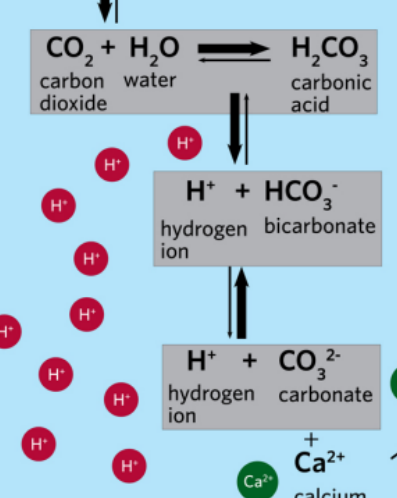
\includegraphics[width=.35\textwidth]{media/SW06.png}
\end{figure*}

\subsection{Question 2}
\pph{How does the structure of benzene contribute to its stability and persistence in the environment?}

Benzene has double and single bonds. This property gives to the chemical a high stability.

Furthermore, having a high volatility, benzene remains in the atmosphere.

\newpage
\subsection{Question 3}
\pph{How does this buffer system limit changes in pH, and why is it becoming less effective?}

This system contains many CO$_2$ molecules that react with water, creating carbonic acid
(H$_2$CO$_3$). Thus, the carbonic acid consumes carbonate (CO$_3^{2-}$) faster than it
creates it.

Increased CO$_2$ in the environment leads to more carbon:
\figbox{\schemestart CaCO$_3$\arrow{<->>}Ca$^{2+}$ + CO$_3^{2-}$ \schemestop}

\subsection{Question 4}
\pph{What chemical and engineering solutions could you propose to mitigate both CO2 and benzene
pollution? -- Name at least 3.}

\begin{itemize}
    \item Reduction in the use of CO$_2$-emitting products;
    \item Implementation of CO$_2$ capture devices in the environment and oceans;
    \item Reduction in the use of pollutants in product manufacturing;
    \item Bio-filtration with algae;
    \item Mitigation of CO$_2$ emissions through the creation of new renewable energy plants;
    \item Increase in the use of solar energy;
    \item Drastic reduction of deforestation and an increase in the number of trees planted;
    \item Preservation of natural sites.
\end{itemize}







\end{document}
